\documentclass[12pt, a4paper]{article} % book, report, article, letter, slides
                                       % letterpaper/a4paper, 10pt/11pt/12pt, twocolumn/twoside/landscape/draft

%%%%%%%%%%%%%%%% PACKAGES %%%%%%%%%%%%%%%%%%%%%

\usepackage[utf8]{inputenc} % encoding

\usepackage[english]{babel} % use special characters and also translates some elements within the document.

\usepackage{amsmath}        % Math
\usepackage{amsthm}         % Math, \newtheorem, \proof, etc
\usepackage{amssymb}        % Math, extended collection
\newtheorem{theorem}{Theorem}[section]
\newtheorem{corollary}{Corollary}[theorem]
\newtheorem{lemma}[theorem]{Lemma}

\usepackage{hyperref}       % Hyperlinks \url{url} or \href{url}{name}

\usepackage{parskip}        % \par starts on left (not idented)

\usepackage{abstract}       % Abstract

\usepackage{tocbibind}      % Adds the bibliography to the table of contents (automatically)

\usepackage{graphicx}       % Images
\graphicspath{ {./images/} }

% \usepackage[document]{ragged2e}  % Left-aligned (whole document)
% \begin{...} ... \end{...}   flushleft, flushright, center

%%%%%%%%%%%%%%%% CODE %%%%%%%%%%%%%%%%%%%%%

\usepackage{minted}         % Code listing
% \mint{html}|<h2>Something <b>here</b></h2>|
% \inputminted{octave}{BitXorMatrix.m}

%\begin{listing}[H]
  %\begin{minted}[xleftmargin=20pt,linenos,bgcolor=codegray]{haskell}
  %\end{minted}
  %\caption{Example of a listing.}
  %\label{lst:example} % You can reference it by \ref{lst:example}
%\end{listing}

\newcommand{\code}[1]{\texttt{#1}} % Define \code{foo.hs} environment

%%%%%%%%%%%%%%%% COLOURS %%%%%%%%%%%%%%%%%%%%%

\usepackage{xcolor}         % Colours \definecolor, \color{codegray}
\definecolor{codegray}{rgb}{0.9, 0.9, 0.9}
% \color{codegray} ... ...
% \textcolor{red}{easily}

%%%%%%%%%%%%%%%% CONFIG %%%%%%%%%%%%%%%%%%%%%

\renewcommand{\absnamepos}{flushleft}
\setlength{\absleftindent}{0pt}
\setlength{\absrightindent}{0pt}

%%%%%%%%%%%%%%%% GLOSSARIES %%%%%%%%%%%%%%%%%%%%%

%\usepackage{glossaries}

%\makeglossaries % before entries

%\newglossaryentry{latex}{
    %name=latex,
    %description={Is a mark up language specially suited
    %for scientific documents}
%}

% Referene to a glossary \gls{latex}
% Print glossaries \printglossaries

%%%%%%%%%%%%%%%% HEADER %%%%%%%%%%%%%%%%%%%%%

\usepackage{fancyhdr}
\pagestyle{fancy}
\fancyhf{}
\rhead{Arnau Abella - MIRI}
\lhead{ADS - First Delivery}
\rfoot{Page \thepage}

%%%%%%%%%%%%%%%% TITLE %%%%%%%%%%%%%%%%%%%%%

\title{%
  Bloom Filter \\
  \large A Simple Implementation In Haskell}
\author{Arnau Abella}
\date{\today}

%%%%%%%%%%%%%%%% DOCUMENT %%%%%%%%%%%%%%%%%%%%%

\begin{document}

\maketitle

\section{Introduction}\label{s:introduction}

A \textbf{Bloom filter} is a space-efficient probabilistic data structure that guarantees constant string comparison with allowable errors \cite{bloom}.

The na\"ive algorithm for string comparison has a computational cost of \\ $\mathcal{O}(m \cdot (n-m+1))$ in time. In contrast, a Bloom filter, performs exact string search in $\mathcal{O}(m+n)$ time by allowing a small probabilistic error. Apart from an excelent computational time, it is also space-efficient and this can be exploited in applications such as dictionaries.

The Bloom filter has a wide range of forms such as Counting Bloom filter or Distributed Bloom filter. And each one has several different applications that we are not going to get in detail.

\begin{figure}[H]
  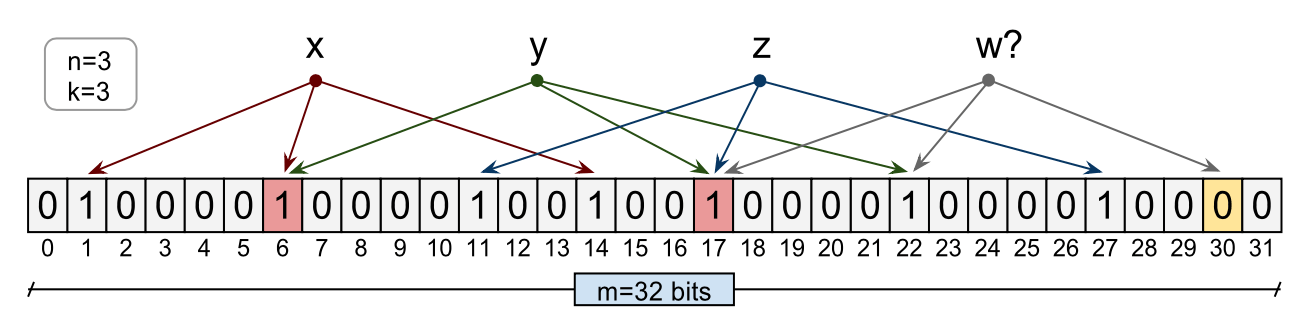
\includegraphics[scale=0.3]{bloom-filter}
  \centering
  \caption{Example of a Bloom filter.}
  \label{fig:bloom}
\end{figure}

A Bloom filter is implemented using an array-like data structure of size $m$ and $H := \{h_1, \dots, h_k\}$ hashing functions, where $h_i := U \to \{0, m-1\}$. Depending on the value of $m$ (size of the array) and $k$ (number of hashing functions), the $\varepsilon$ (expected error rate) will be different. The algorithm has the following steps:

\begin{enumerate}
  \item Initialize an array of size $m$ to 0.
  \item On each new string, hash it using $h_{\in H}$ and add one to the corresponding index in the array.
  \item Given a new word, hash it again using $h_{\in H}$ and check if their corresponding indexes are 1 in the array. If all indexes' positions are set to 1, you have a high probability that the word has been already searched. Otherwise, you are guaranteed that the word has not been searched and you can add it to the array.
  \item (Optional) At some point, $70-80\%$ of the positions of the array will be one, so the bloom filter will not work properly. You can implement a \code{reset} method to restart the data structure setting all bits to zero.
  \item (Optional) You can have multiple layers to check if the word has been searches $n$ times.
\end{enumerate}

This process is illustrated in the figure \ref{fig:bloom}.

\subsection{Probability of the error rate}\label{s:probability}

This section explains formally the $\varepsilon$ (expected error rate) $wrt.$ the independent variables $m$ (array size), $n$ (number of strings present in the filter), and $k$ (number of hashing functions).

\begin{itemize}
  \item The probability of setting a bit is $1/m$. This comes from the assumption that $H$ belongs to the class of Universal Hashing Functions.
  \item The probability of not setting a bit to 1 is $1 - 1/m$.
  \item The probability of not setting a bit to 1 after the $k$ hashing functions is $(1 - 1/m)^k$.
  \item The probability of not setting a bit to 1 after $k$ hashing functions and $n$ strings is $(1 - 1/m)^{kn}$.
  \item The probability of mistaken a bit is $1 - (1 - 1/m)^{kn}$
  \item And error is produced when we mistake the $k$ indexes of a string and the probability is $(1 - (1 - 1/m)^{kn})^k$.
  \item This can be approximated by $1 - e^{-kn/m}$
\end{itemize}

From the formula of the error rate

\[
  \varepsilon = 1 - e^{-kn/m}
\]

it is easy to appreciate that when $m \to \infty^+$, $\varepsilon \to 0$. So, $m$ should be big. But, how big ?

Before answering this question, we should note that there is an optimal $k$ value where the function $p = e^{-kn/m}$ is minimal. This can be computed differentiating the equation and equating it to zero. The optimal $k$ can be found by the formula:

\[
  k = \frac{m}{n}\log_{} 2
\]

As we said, the size of $m$ depends on $n$ (but this is fixed by the problem), $k$ (but we found that there is an optimal one) and $\varepsilon$. Now, the size of $m$ only depends on the error rate and it can be computed this way:

\[
  m = \lceil \frac{\log \frac{1}{\varepsilon} \cdot n}{\log^2 2} \rceil
\]

Notice that the error rate is only influence by the FPR (false positives rate) as it is guarantee that there are no false negatives.

\section{Experiment}\label{s:experiment}

The experiment for this delivery consist of empirically proving that the implementation proposed in this delivery of a Bloom filter in Haskell, which uses the previous formulas, has the expected theoretically error rates.

The experiment is quite simple and it is implemented in the following steps:

\begin{itemize}
  \item For $n = \langle 100, 1000, 10000\rangle$:
  \item For $\varepsilon = \langle 0.05, 0.01, 0.001\rangle$:
  \item For $i = \{0..100\}$:
  \item Generate $n$ strings,
  \item construct a Bloom filter using the $n$ strings,
  \item then, test it against $m \sim n$ new strings,
  \item and collect if the test was a true positive, a false positive, a true negative or a false negative.
  \item This process is repeated $i$ times to improve the quality of the test and it is a probabilistic data structure.
  \item Finally, output the results for each $n$ and $\varepsilon$.
\end{itemize}

\begin{listing}[H]
  \begin{minted}[xleftmargin=0pt]{haskell}
-- | Runs an error rate test
-- and writes the result at the given file path.
errorRateTest :: FilePath -> IO ()
errorRateTest file =
  withFile file WriteMode $ \h -> do
    forM_ [100, 1000, 10000] $ \n -> do
      forM_ [0.05, 0.01, 0.001] $ \e -> do
        (fp, fn) <- fmap unzip $ forM [0..100] $
            \(_ :: Int) -> do
              samples' <- generate (genSamples n)
              let (trainingSet, testingSet) =
                coerce @_ @([String], [String]) samples'
              let !filt = BF.create e trainingSet
              let wrds = Set.fromList trainingSet
              let (l, r) = foldr (testFilt filt wrds) (0,0) testingSet
              let overN x = (fromIntegral x) / (fromIntegral n) :: Double
              return (overN l, overN r)
        let (fpr, fnr) = (mean fp, mean fn)
        let (sfp, sfn) = (stdDev fp, stdDev fn)
        _ <- traverse (hPutStrLn h) [ "False Positive Rate"
                                    , "mean      = " ++ show fpr
                                    , "std. dev. = " ++ show sfp
                                    , "False Negative Rate"
                                    , "mean      = " ++ show fnr
                                    , "std. dev. = " ++ show sfn
                                    ]
  \end{minted}
  \caption{Error rate test implementation}
  \label{lst:error-rate-test}
\end{listing}

\newpage

The output of the experiment for $\varepsilon = 0.05$ and $n = \{100, 1000, 10000\}$ is the following:

\begin{listing}[H]
  \begin{minted}[xleftmargin=0pt]{haskell}
N = 100
Expected e = 5.0e-2

False Positive Rate
	mean = 6.0e-3
	std. dev. = 1.5e-4

False Negative Rate
	mean = 0.0
	std. dev. = NaN

-----------------------------

N = 1000
Expected e = 5.0e-2

False Positive Rate
	mean = 1.4e-3
	std. dev. = 1.65e-4

False Negative Rate
	mean = 0.0
	std. dev. = NaN

-----------------------------

N = 10000
Expected e = 1.0e-2

False Positive Rate
	mean = 5.4e-3
	std. dev. = 1.2e-4

False Negative Rate
	mean = 0.0
	std. dev. = NaN
  \end{minted}
  \caption{Output of the experiment for $\varepsilon = 0.05$}
  \label{lst:test-output}
\end{listing}


\section{Conclusion}\label{s:conclusion}

We presented an implementation of the most simple version of a Bloom filter written in Haskell with an efficient-space representation and reasonable performance. We proved by experimentation that, in practice, the theoretical error rate holds.

In the future, this data structure can be extended to support concurrent and distributed computation.

%%%%%%%%%%%%%%%% BIBLIOGRAPHY %%%%%%%%%%%%%%%%%%%%%

\bibliographystyle{unsrt} % abbrv, aplha, plain, abstract, apa, unsrt,
\bibliography{refs}

\end{document}
